\chapter{REVISÃO DE LITERATURA}
\label{chp:capitulo3}
Em um campo com artigos, publicações e materiais em larga parte espalhados por blogs na internet, foi necessário realizar uma revisão de literatura para que as ferramentas de ponta, estratégias ainda sendo testadas e vulnerabilidades principais no mercado fossem corretamente identificadas. Isso se torna especialmente verdadeiro pela mudança no cenário de segurança dos anos 2000 para os anos 2010-2022, aonde boa parte de ameaças antigas podem ser de pouca relevância.

Neste capítulo estão alguns dos principais achados.

\section{Avaliação de Propostas de Segurança para Aplicações Web}
Ao fim da coleta de artigos, além do embasamento teórico e melhor enquadramento do escopo a ser estudado, buscou-se uma série de ferramentas e/ou casos reais de modelos e sistemas sugeridos na área de segurança da informação em sistemas Web, para que um desses pudesse ser expandido.

\subsection{nscanner}
Essa solução, publicada apenas na forma de um artigo \cite{surian_nscanner_2020}, provém de um estudo dirigido sobre uma série de outras ferramentas existentes hoje no mundo de segurança da informação (e de utilidade/notoriedade no mercado) como \textit{Metasploit}, \textit{Wapiti} e \textit{Acunetix}. O nscanner agrupa essas ferramentas e usa cada uma delas em determinadas partes de seu funcionamento, assim ganhando relevância por ter uma funcionalidade mais ampla.  Trata-se de uma aplicação dinâmica, flexível e automatizada para detectar os ataques mais comuns e problemáticos em segurança de Informação, que são injeções SQL e \textit{Cross Site Scripting}. É capaz também de detectar malware via Aprendizado de Máquina para prevenir resultados que seriam falsos positivos ou negativos.

Há uma fase de testagem de vulnerabilidade em aplicação Web. Uma etapa independente permite o escaneamento de arquivos supostamente maliciosos fornecidos pelo usuário para detecção de malware. Todas as informações trabalhadas são armazenadas localmente, tornando desnecessário o uso de uma solução de Banco de Dados, que seria tipicamente usada com uma ferramenta dessa natureza.

Para a primeira fase, as seguintes etapas são observadas pelo autor:
\begin{alineas}
\item Tendo sido estabelecida uma conexão com a internet, um usuário da ferramenta escolhe o tipo de vulnerabilidade que será testada (se é injeção SQL ou \textit{Cross Site Scripting}). Após isso, ele fornece um endereço web ou de IP que armazena a aplicação que receberá os testes. Não é especificado pelos autores se há suporte a todos os protocolos HTTP/1.1, /2, /3, ou HTTPS, porém idealmente a aplicação suportaria todos.
\item Uma requisição com os dados fornecidos pelo usuário é feita ao web \textit{crawler} do Nscanner, um script responsável por acessar a aplicação em si e realizar a verificação por vulnerabilidades. Ele busca o site da aplicação pelo domínio, usado para identificar o servidor armazenando tal site.
\item Após isso, uma conexão com o servidor encontrado é requisitada pelo \textit{crawler}, estabelecendo então uma ponte entre web \textit{crawler} e servidor. Assim as páginas e componentes da aplicação em análise são navegadas e todas as partes com formulários são identificadas.
\item Nessa etapa (a mais importante da pipeline), os bugs são identificados pelo Nscanner. A ferramenta injeta entradas de acordo com a seleção de vulnerabilidade do usuário no início do fluxo, em todas as partes críticas (formulários) visualizadas na análise anteriormente feita a fim de verificar se alguma delas omite erros fundamentais deixando passar uma vulnerabilidade. Espera-se um tempo de processamento não desprezível por ser um processo iterativo. Finalmente é gerado um relatório que o usuário final pode optar por baixar para fins de histórico ou apenas visualizar no momento.
\end{alineas}

Enfim tem-se a segunda parte da proposta, de escaneamento de arquivos:
\begin{alineas}
\item É feito um upload de um arquivo/amostra que o usuário considera malicioso ou suspeito ao Nscanner. Um critério para essa suspeita pode ser análise do código fonte desse arquivo que mostre etapas que possam comprometer uma aplicação, um pacote com conteúdo que pareça estar buscando se aproveitar de vulnerabilidades e assim por diante. 
\item O principal componente da detecção de malware do Nscanner é acionado ao verificar que o upload foi bem sucedido, iniciando uma análise dinâmica. Por exemplo, um classificador de Aprendizado de Máquina baseado no algoritmo de \textit{Random Forest}, treinado para detectar arquivos malware com uma série árvore de decisões geradas em seu treinamento pode ser usado. Verificando com sucesso algum caso em que a precisão seja suficiente para definir como malicioso, o arquivo é designado como tal e um relatório é gerado semelhantemente a etapa anterior para o usuário.
\end{alineas}

Embora seja um projeto conveniente, do qual a ideia de utilizar um classificador para detecção de vulnerabilidades pode ser muito aproveitada,  percebem-se algumas falhas nessa implementação. 

Em particular, na etapa mais importante do fluxo de detecção de vulnerabilidades em aplicação web, há pontos críticos que o autor não cuidou de verificar: não há uma proposta suficientemente concreta para fornecer entradas que testem a aplicação corretamente nesse fluxo. Este processo, que é bastante complexo, existe em algumas aplicações no mercado. Além disso, a diferença entre injeções SQL e \textit{Cross Site Scripting} (XSS) não garante necessariamente  que as vulnerabilidades aparecerão nos mesmos pontos críticos da aplicação. É frequente observar vulnerabilidades XSS em partes até impossíveis de se realizar injeções SQL.

Como esta proposta é apenas uma ideia sem implementação e considerando as questões críticas apontadas acima, foi descartada a expansão desta proposta dentro do escopo pretendido pelo trabalho.

\subsection{GraphXSS}
A proposta do GraphXSS \cite{liu_graphxss_2022} sugere uma implementação de uma Rede Convolucional de Grafos (em inglês: \textit{Graph Convolutional Network}, abreviado como GCN) para realizar a detecção de ataques de \textit{Cross-Site Scripting} (explicado anteriormente na Seção 2.2) em aplicações web. A \textit{pipeline} básica envolve um pré-processamento dos dados, a composição dos mesmos em uma estrutura de grafos, e a utilização de algoritmos que realizam \textit{Deep Learning} em cima dessa estrutura para enfim realizar a detecção de maliciosidade em uma determinada entrada. A solução é mostrada no diagrama da Figura 5: 

\begin{figure}[H]
    \centering
    \caption{Arquitetura do Sistema GraphXSS proposto}
    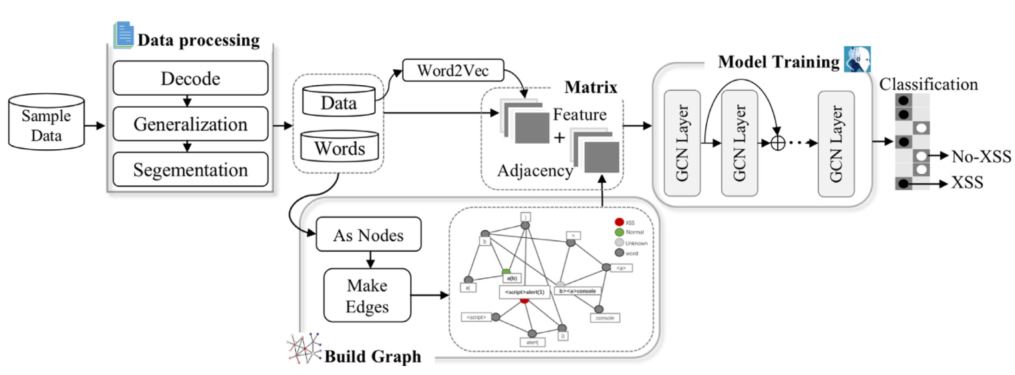
\includegraphics[width=14cm]{figuras/graphXSS.png} 
    \legend{Fonte: \href{https://www.sciencedirect.com/science/article/pii/S016740482100420X}{Z. Liu, Y.Fang, C. Huang et al via Scopus} (2022)}
    \label{fig:internet} 
\end{figure}

O pré-processamento do bloco inicial \textit{Data Processing} da arquitetura mostrada na Figura 5 tem por finalidade reduzir a parametrização excessiva, técnica na qual os parâmetros do algoritmo são mais numerosos do que os próprios dados de treinamento. Os autores acreditam que essa técnica possa interferir com os resultados finais de detecção do sistema.

Com a realização dessa etapa, também se obtém uma redução no custo computacional de subsequentes treinamentos efetuados nas etapas de classificação (justamente o momento mais exigente do sistema), melhorando também a eficiência do algoritmo. No bloco \textit{Decode}, localizado após \textit{Sample Data} na Figura 5, são utilizados algoritmos comuns de encodificação/decodificação como primeira etapa, compreendidos por: \textit{URL decoding}, \textit{HTML entity encoding}, \textit{Unicode decoding} e \textit{Base64 decoding} para decodificação. Os resultados destes quatro algoritmos são generalizados (via discretização, generalização e/ou padronização de dados) e segmentados no Tokenizador de expressões regulares do módulo NLTK (\textit{Nature Language Toolkit}).

Como mostrado na Figura 5, este pré-processamento dá entrada no módulo de composição para grafo, responsável por conectar palavras e dados de uma maneira regular para formar um grafo dotado de \textit{data points} (no caso, um tipo de nó) e arestas. Esse grafo é formado para uso no módulo de \textit{Deep Learning} (baseado em algoritmos de GCNs e mostrado no bloco \textit{Model Training na Figura 5}) que otimiza seus parâmetros. Finalmente, após o treinamento inicial, obtém-se uma distribuição de probabilidade de cada vértice que levará à classificação do \textit{data point} fornecido ao sistema. 

Em comparação com as demais soluções levantadas, essa arquitetura não trabalha com injeções SQL em nenhuma forma, não oferece a usuários finais uma solução acionável e tem alta complexidade. Muitos dos detalhes da implementação do GraphXSS, com exceção dos diagramas da arquitetura geral  e das saídas da etapa de classificação final, não foram encontrados nas referências, tornando também impossível o aproveitamento  desta ferramenta para a extensão pretendida no trabalho realizado. 

% Espera-se que algum dia os autores disponibilizem um repositório com os códigos da experimentação realizada, ou talvez uma implementação mais concreta que seja mais factível para alunos e entusiastas contribuírem.

\subsection{PADRES}

O PADRES \cite{pereira_padres_2022}, sigla para PrivAcy, Data REgulation and Security, é um software desenvolvido inicialmente para auxiliar a infraestrutura do EPOS (\textit{European Plate Observatory System}) e a comunidade do GNSS (\textbf{Global Navigation Satellite System}) em um ponto pouco explorado em Segurança da Informação no contexto de Internet - complacência com a GDPR (\textit{General Data Protection Regulation}), uma regulação introduzida em 2016 na legislatura Europeia com finalidade de proteger a privacidade e acesso aos dados alheios. Porém sua solução tornou-se generalizada o suficiente para auxiliar empresas de escopos variados, servindo para qualquer aplicação Web que seja aberta. A parte de interesse do PADRES é a funcionalidade embutida de analisar aplicações Web por vulnerabilidades, dado que privacidade de dados é comumente associada com segurança.

O fluxo básico dessa aplicação envolve o usuário fornecer um endereço de uma aplicação Web a ser analisada, seguido de uma série de perguntas sobre GDPR que são respondidas manualmente pelo administrador da mesma. Com isso, a aplicação é analisada pelo PADRES, e um relatório sobre suas vulnerabilidades e pendências com a regulação GDPR (baseadas nas respostas fornecidas no questionário manual) é disponibilizado para baixar. 

A Figura 6 é uma captura de tela do PADRES em funcionamento, em sua tela inicial mostrando opções de seleção de país e de software para ser analisado.

\begin{figure}[ht]
    \centering
    \caption{Screenshot do PADRES em funcionamento}
    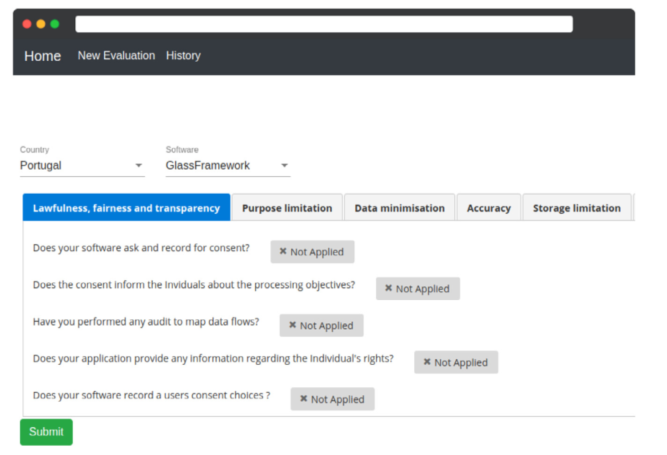
\includegraphics[width=14cm]{figuras/padres.png} 
    \legend{Fonte: \href{https://www.sciencedirect.com/science/article/pii/S2352711021001515}{Fábio Pereira, Paul Crocker, Valderi R.Q. Leithardt et al via Scopus} (2022)}
    \label{fig:internet} 
\end{figure}

Em termos de arquitetura, o PADRES é dotado de um modelo de Cliente e Servidor. Há um \textit{front-end} desenvolvido no framework Angular (para JavaScript), e o \textit{back-end} implementa uma arquitetura REST por meio do framework Flask, em \textit{Python}. Um banco de dados preenchido de questões GDPR a serem respondidas é conectado ao \textit{back-end}, e uma estrutura para armazenar metadados do relatório final em formato \verb+.blob+ é providenciada. Esse banco é modelado de maneira que as perguntas são extensíveis, tornando o software um bom candidato para expansão. Algumas ferramentas de código aberto de \textit{Penetration Testing} são utilizadas no módulo de detecção de vulnerabilidades Web, são elas: Wapiti, ZAP e NMAP. Elas são executadas pelo usuário via a interface gráfica, com suas saídas sendo acopladas à saída do questionário GDPR.

Todo esse arcabouço técnico é encapsulado pelo Docker, a principal ferramenta de conteinerização de software hoje no mercado, escrita em Golang. Através desse artifício, qualquer sistema operacional utilizando Docker consegue instalar o ambiente de desenvolvimento sem problemas e executar a aplicação.

Esse e o fato da extensibilidade da aplicação ser algo muito enfatizado pelos autores fez do PADRES uma opção inicial para a extensão pretendida pelo trabalho. Todavia, uma série de dificuldades imprevistas foram encontradas. Não só o repositório com a aplicação fornecida carecia gravemente de documentação, como a aplicação no estado atual não funcionou como previsto em uma variedade de ambientes testados. Apenas um esqueleto do \textit{front-end} é corretamente disponibilizado, porém a parte da interface gráfica responsável por selecionar uma aplicação Web de fato encontrava-se impossível de ser selecionada. Algumas estratégias para contornar isso foram tentadas, porém sem sucesso. Não foi encontrada também uma forma de verificar o correto funcionamento do \textit{back-end}.

Com isso o PADRES no estado atual não pode ser recomendado como uma ferramenta operacionalmente viável, mesmo que sua ideia resgate interesses de privacidade de alta relevância, até mesmo fora da Europa, e reforce a importância de documentação e testagem robusta de aplicações que sejam criadas com o intuito de reforçar software no geral. 
% Tanto o \textit{wafamole++} como o software \textit{WAF-A-MoLE} no qual foi baseado possuem documentação suficiente e funcionamento pleno para serem notáveis como contribuições para a comunidade de Segurança da Informação.

\subsection{WAF-A-MoLE}

Desenvolvido como uma tese, o \textit{WAF-A-MoLE} \cite{valenza_waf--mole_2020} é uma ferramenta geradora de testes para WAFs baseados em Aprendizado de Máquina. A versão atual é particularmente dedicada a injeções SQL. Sendo um dos poucos softwares encontrados nos artigos com uma implementação concreta (a outra sendo o PADRES, que mostrou-se defeituosa), o \textit{WAF-A-MoLE} certamente foi um dos mais convidativos a colaboração. Não só os autores providenciam uma documentação robusta para uma aplicação inicialmente desenvolvida no meio acadêmico, como também mostram nela caminhos a serem expandidos por contribuintes futuros.

\begin{figure}[ht]
    \centering
    \caption{Arquitetura do \textit{WAF-A-MoLE} - $p_i$ indica entrada (do inglês \textit{payload}) i e $\sigma_i$  indica pontuação (do inglês \textit{score}) de confiança i.}
    % $num_{\mathrm{expression}}$ for n+1 subscript!
    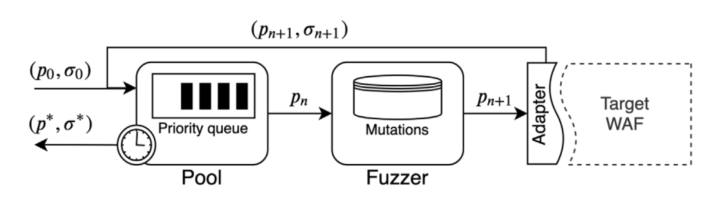
\includegraphics[width=14cm]{figuras/wafamoleArchitecture.png} 
    \legend{Fonte: \href{https://arxiv.org/abs/2001.01952}{A. Valenza, L. Demetrio, G. Costa and G. Lagorio et al via arxiv} (2020)}
    \label{fig:internet} 
\end{figure}


A arquitetura do \textit{WAF-A-MoLE} é mostrada na Figura 7. Ela consiste do bloco \verb+Pool+, uma fila com prioridade, do bloco \verb+Fuzzer+, que implementa mutações, e da classe \verb+Adapter+, comentados a seguir. 

Inteiramente codificado na linguagem de programação \textit{Python 3}, esse software faz uso de uma metodologia de testagem baseada em \textit{fuzzing} (inspirada pelo \textit{Fuzzing Book}) \cite{fuzzing_book} para criar ataques que penetrem com sucesso um determinado WAF baseado em Aprendizado de Máquina a ser analisado. Mais precisamente, fazendo uso da pontuação de classificação do WAF como métrica, o processo de \textit{fuzzing} é guiado de maneira que as entradas mais promissoras são priorizadas.

Ele é implementado como uma biblioteca e como uma ferramenta de linha de comando, por meio de \textit{Click decorators} (uma função da biblioteca \textit{Click} para minimizar o código por trás de aplicações de linha de comando). O usuário pode escolher qual modelo será utilizado, além de uma série de parâmetros como \verb+timeout+, rodadas máximas \footnote{Rodadas máximas: Número máximo de iterações a serem realizadas}, caminho para o arquivo de saída e afins.

Tomando como base a figura de sua arquitetura acima, seu funcionamento é iniciado com uma entrada (\textit{payload}) inicial $p_0$ (fornecido pelo usuário ao executar o programa) ao qual o WAF a ser testado confere uma pontuação de confiança $\sigma_0 \epsilon [0, 1]$ que será inserido em \verb+Pool+, uma estrutura contendo entradas. Essa estrutura \verb+Pool+ é uma fila de prioridade que armazenará entradas subsequentes por ordem decrescente de suas pontuações de confiança, de modo que as entradas com menor pontuação de confiança terão maior prioridade de saída.

Com isso, a cada iteração a cabeça da fila $p_n$ é selecionada pela \verb+Pool+, passada adiante para a classe \verb+Fuzzer+, que realiza uma mutação em cima de $p_n$ transformando-o em $p_{\mathrm{n+1}}$, aplicando aleatoriamente um dos operadores de mutação padrões do programa (A lista completa de operadores de mutação pode ser conferida nos apêndices). $p_{\mathrm{n+1}}$ é submetido então ao WAF alvo para classificação/avaliação e sua pontuação de confiança é gerada por uma classe \verb+Adapter+ após isso. A natureza extensível do \textit{WAF-A-MoLE} permite que uma variedade de WAFs sejam testados desde que estejam com adaptadores específicos para garantir compatibilidade. A classe \verb+Adapter+ retorna então a pontuação de $\sigma_{\mathrm{n+1}}$ de $p_{\mathrm{n+1}}$, sendo colocado de volta na fila \verb+Pool+ de entradas para sofrer novas mutações nas próximas iterações.

\bigskip 

Com esse funcionamento, a condição de parada é dada da seguinte forma:
\begin{alineas}
\item No momento em que uma pontuação de confiança $\sigma^*$ é menor do que um limite dado pelo usuário no início do programa (no parâmetro \verb+threshold+) - retorna-se o melhor par ($p^*, \sigma^*$) encontrado;
\item Caso o número de iterações máximas seja atingido e nenhuma pontuação de confiança $\sigma^*$ menor que \verb+threshold+ seja encontrada, o par ($p^*, \sigma^*$) mais próximo do mesmo é retornado;
\item O programa é interrompido via \verb+SIGKILL+, \verb+SIGTERM+ ou semelhante.
\end{alineas}

\bigskip

Para testagem de WAFs de diferentes origens e arquiteturas, uma classe \verb+Model+ é disponibilizada pelos autores como uma interface, generalizando o comportamento de modelos usados. Assim, o componente amostrado na Figura 7 como \textit{Adapter} ao lado de \textit{Target WAF} pode ser criado a partir dessa classe. Ao adaptar um WAF para ser testado, o desenvolvedor precisa compará-las com os adaptadores dos modelos de exemplo do \textit{WAF-A-MoLE} para saber quais características são usadas pelo mesmo no funcionamento de sua arquitetura.

% Para testagem de WAFs de diferentes origens e arquiteturas, uma classe \verb+Model+ é disponibilizada pelos autores como uma interface, generalizando o comportamento de modelos usados. Dois métodos abstratos \verb+classify+ e \verb+extract_features+ são instanciados para cada modelo. Ao adaptar um WAF para ser testado, o desenvolvedor precisa buscar as funções equivalentes de seu classificador interno e compará-las com os modelos de exemplo do \textit{WAF-A-MoLE} para saber quais características são usadas pelo mesmo no funcionamento de sua arquitetura.

Essa necessidade de experimentação para adaptação não se mostrou muito clara, porém foi possível (com a ajuda dos autores originais) construir um \textit{wrapper}/interface geral para modelos do \verb+scikit-learn+ com o \textit{wafamole++} - a extensão desse software melhor detalhada nos capítulos 4 e 5 deste documento.

\subsection{Conclusão}
Em suma, percebe-se que o \textit{WAF-A-MoLE} é uma excelente ferramenta base para reforçar WAFs baseados em Aprendizado de Máquina. Configurando rotinas para gerar uma série de exemplos adversariais a partir do mesmo, especialistas de segurança podem refazer o treinamento de seus \textit{Firewalls} complementando seus exemplos de base com os adversariais recém-gerados, chegando a níveis de robustez mais aceitáveis. 

Entretanto, não é uma solução sem imperfeições, das quais podem ser destacadas:
\begin{alineas}
\item Uma falha na documentação de suas dependências (em particular quanto à versões);
\item A arquitetura se mostrou engessada para adaptar para modelos novos, mesmo com incentivo pelos autores originais;
\item Muitos dos detalhes de treinamento de dados se mostraram ofuscados na documentação, juntamente de estruturas de dados usadas em seu funcionamento.
\end{alineas}

Por esses motivos foi decidida a extensão do mesmo, nomeada de \textit{wafamole++}, a fim de amenizar as dificuldades encontradas na sua execução e enriquecer seu funcionamento para futuros desenvolvedores e profissionais de segurança.


